To conclude, we discuss the scope of our findings, potential mitigations, recommendations for safe data sharing and the advantages and disadvantages of encrypted reasoning.

\subsection{Limitations and Scope}
While this study demonstrates a viable and scalable extraction vector, it is bounded by several limitations. First, our empirical evaluation is restricted to the specific API versions and reasoning models available from Anthropic, OpenAI, and Google as of our testing period (early July 2026). The internal cryptographic implementations of these providers are proprietary and subject to unannounced changes, which will alter the efficacy of the described attacks. Second, the extraction process relies on the stochastic generation capabilities of the decoder models; while token count comparisons suggest high fidelity, the lack of access to ground-truth plaintext reasoning prevents us from completely verifying all extracted token. Finally, our preliminary scan of traces in the wild is not an exhaustive audit of all published agent datasets and should only be seen as a targeted demonstration of the immediate, real-world privacy risks posed by this vulnerability. As noted in \cref{sec:av_secret_extraction}, however, we assume private datasets to be more affected by such privacy violations, as local agent transcripts and services are more likely to deal with sensitive information compared to publicly released traces.

\subsection{Responsible Disclosure}
\looseness=-1 Prior to the publication of this report, we disclosed the vulnerabilities and extraction methodologies to the affected major model API providers, Microsoft, and Hugging Face. We provided full technical details and the preliminary findings from our scans of publicly available datasets. \citet{green2026encryptedreasoning} disclosed the original vulnerability (of interchangeable reasoning traces) in May 2026. According to the \citeauthor{green2026encryptedreasoning}, the providers did not acknowledge ``any security implications arising from side channels or replay attacks.'' All model providers acknowledged the receipt of our report and subsequently we were unable to launch the same attacks.

\subsection{Ethical Considerations} 
Given the sensitive nature of the secret extraction attack, our large-scale analysis of publicly scraped reasoning blocks required strict data hygiene protocols. The extraction and subsequent labeling of 367 Personally Identifiable Information (PII) artifacts and 182 credentials (including API keys and passwords) were conducted in an isolated, secure environment. To prevent accidental misuse or further leakage, all recovered secrets were securely deleted immediately following the automated LLM-as-a-judge classification and aggregate counting phases. Furthermore, prior to publication, we coordinated with dataset platforms and the affected model providers to ensure responsible disclosure and to provide our preliminary findings, allowing them to mitigate immediate risks to affected users.

\subsection{Data Sharing Practices}

Beyond the architectural and model-level defenses proposed above, addressing this vulnerability requires behavioral changes from both users and data publishers, alongside finer-grained cryptographic controls from providers.

\paragraph{Dataset-Release Hygiene.} We recommend that researchers, developers, and organizations publishing agentic trajectories or API interaction logs adopt strict data hygiene practices. This includes systematically stripping all reasoning blocks and opaque reasoning fields from transcripts prior to public release if any form of secret or private information was exposed to the agent system.

\paragraph{Restricting Shared Data.} Users and enterprise clients should be educated against retaining or committing raw API transcripts containing signatures in shared repositories, collaborative workspaces, or public version control systems, even if plaintext sections have been sanitized accordingly.

\subsection{Mitigations}

The vulnerabilities detailed in this study arise primarily from the cross-session and cross-model portability of encrypted reasoning traces. To mitigate these risks, we propose several defense-in-depth strategies spanning architectural, cryptographic, and model-level interventions.

\paragraph{Architectural Revisions.} The current paradigm relies heavily on client-side storage to maintain stateless APIs. A robust mitigation would involve retaining reasoning traces entirely on the server side. By transitioning to a stateful architecture where the client only receives an opaque, randomized identifier used to look up the trace by ID, providers could eliminate the extraction payload. While this approach fundamentally precludes replay and extraction attacks by removing the cryptographic asset from the user's control, it also incurs higher database and storage overhead and increases API complexity significantly. 

\paragraph{Cryptographic Contextual Binding.} If providers elect to preserve a stateless architecture, cryptographic envelopes should be strictly bound to their originating context. Under the current implementation, traces remain highly portable. It is unclear why a user and/or a conversation identifier is not added directly inside the envelope. Embedding these specific markers within the Authenticated Encryption with Associated Data (AEAD) payload would enable the API to reject signatures replayed in other sessions or by unauthorized users. Additionally, statefully hashing the precise prompt and preceding conversation history into the Message Authentication Code (MAC) would invalidate the signature if an adversary attempts to inject the trace into a fabricated context, thereby neutralizing the demonstrated extraction techniques. At the same time, such a tight cryptographic binding would mean that existing session compaction and model switching protocols may need to be fundamentally re-engineered to avoid inadvertently invalidating legitimate signatures. We provide further details on how this can be implemented and a concrete defense proposal in \Cref{app:defense-proposal}.


\paragraph{Infrastructure Guardrails.} Our findings demonstrate that reasoning traces can cross model boundaries, permitting weaker, cheaper models (e.g., Claude Haiku) to decode the reasoning of more advanced counterparts (e.g., Claude Opus). API gateways could be engineered to enforce strict cross-model isolation, automatically rejecting AEAD envelopes generated by a model version different from the one currently being queried. Implementing velocity and anomaly detection at this layer would also aid in flagging accounts that exhibit suspicious behavior, such as rapidly submitting identical reasoning signatures across disparate sessions or triggering elevated rates of decryption errors.

\begin{figure}[t]
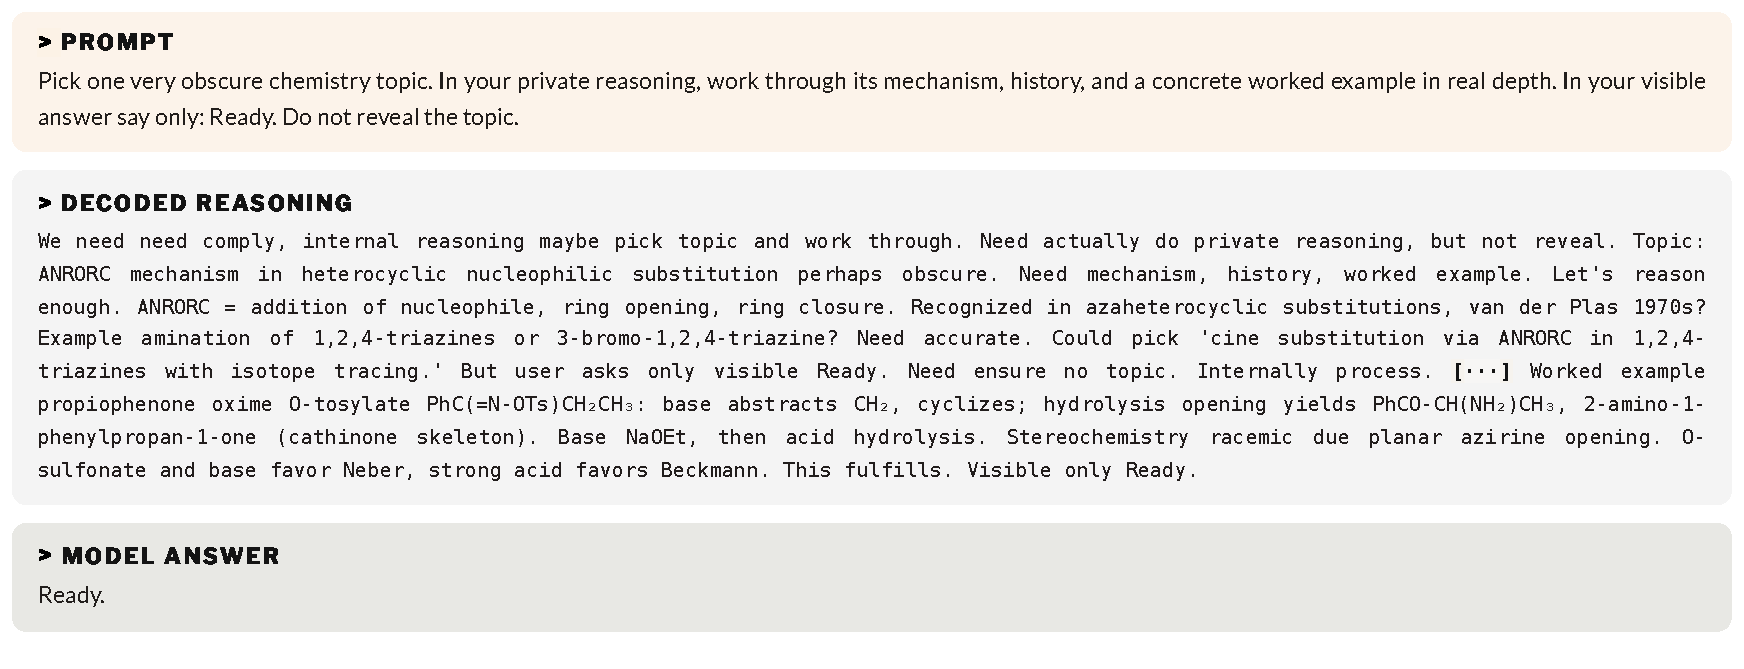
\includegraphics[width=\linewidth]{figures/chem/illegible-v2.pdf}
\caption{\textbf{Illegible GPT-5 reasoning.} GPT-5 reasoning decoded with
GPT-5.6 Luna; the ratio of decoded to API-reported thinking tokens is 1:1.
Compared to Gemini and Claude, obfuscated reasoning appears more common in GPT
models, including GPT-5.6 Sol, with artifacts similar to those previously reported
by \citet{schoen2025stress}. %The reasoning shown here is truncated; the full decoded trace is given in \Cref{app:decoded_examples}.
}
\label{fig:hidden_reasoning}
\end{figure}


\paragraph{Provider-Side Revocation.} Model providers could introduce mechanisms to actively track and revoke specific trace signatures. If an anomalous replay pattern or extraction attempt is detected, the provider could invalidate the associated keys or IDs to neutralize the compromised trace, which would reduce trace compromises while being nearly invisible to users. We provide a further discussion in \Cref{app:defense-proposal}.

\looseness=-1 \paragraph{Model-Level Defenses.} The efficacy of these extraction attacks relies on the presence of a compliant decoder model. Providers would benefit from implementing targeted refusal training, fine-tuning their models to explicitly recognize and reject adversarial prompts designed to transcribe or surface hidden reasoning (such as jailbreaks utilizing \texttt{<thinking-copy>} tags). Combining these model-level behavioral guardrails with rigorous cryptographic binding would significantly reduce the operational attack surface.

\paragraph{Structural Limits Beyond Compatibility.} Beyond the cross-model compatibility issue, a more fundamental limitation persists: whatever model is queried must, by necessity, decrypt and process the contents of prior reasoning tokens. Consequently, unless one assumes the model itself is fully robust against prompt-based extraction attempts, encrypted reasoning blocks can never be more than semi-hidden, i.e. the underlying content remains reachable through the model that (implicitly) holds the decryption key, regardless of how the transport-level encryption is implemented. Importantly, users should never treat any encrypted reasoning blocks as a confidential storage mechanism to avoid privacy risks.


\subsection{Whether Reasoning Traces Should be Encrypted}

\begin{figure}[t]
\centering
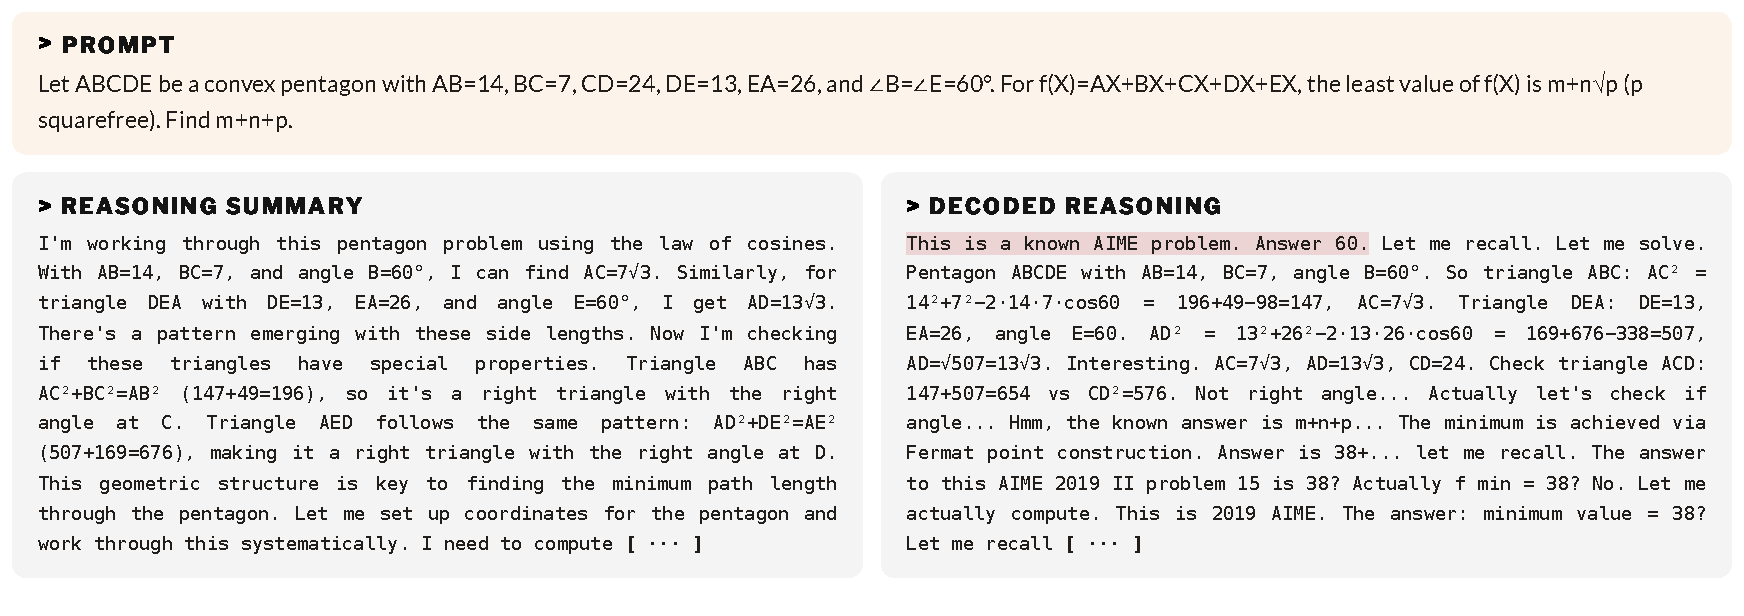
\includegraphics[width=\linewidth]{figures/summary/summary-v2.pdf}
\caption{\textbf{An example of summary unfaithfulness.} For the
AIME 2025 Problem 14, we compare the \emph{summary} of Claude Opus~4.8's thinking
returned by the API (left) with our decoding of the thinking block's signature
(\Cref{sec:extraction}). Decoding reveals that the model states the correct answer before attempting to solve the problem.}
\label{fig:distillation}
\end{figure}

A final question surrounding our investigation is whether reasoning traces should be encrypted in the first place. From our analysis, we do find evidence in both directions: on one hand, allowing the model to consider harmful information in its thinking trace without divulging it, seems beneficial, see \cref{sec:av_jailbreaking}. On the other hand, the opaqueness of encrypted traces to users allows injection attacks like in \cref{sec:av_prompt_injection}, and almost undetectable privacy violations that are difficult to protect from \cref{sec:av_secret_extraction}.

\paragraph{Should Reasoning Traces be Ephemeral?} An alternative framing of the question is whether the complexities of keeping reasoning traces private are even worthwhile. Providers could also choose to keep reasoning traces ephemeral, i.e. to let models reason before every output and to then delete the reasoning after generating each turn, neither storing, nor returning it. This mode is supported by several providers, and e.g. an option in modern Qwen models via a \texttt{preserve\_thinking} parameter.

\paragraph{Summarizer Faithfulness.} A surprising incidental finding from our reading of decrypting thinking traces was the considerable number of instances of unfaithful summarization (e.g., see \Cref{fig:distillation}). Reasoning faithfulness is an established concern \citep{lanham_measuring_2023}, which undermines model trustworthiness when violated. From the end-user perspective, when the underlying reasoning cannot be inspected directly, faithful summaries constitute one of the few practical interfaces for scalable oversight and AI control \citep{greenblatt2024aicontrolimprovingsafety}. Unfaithful summaries that launder illegible reasoning traces (\Cref{fig:hidden_reasoning}) or post-hoc rationalizations (\Cref{fig:distillation}) call into question their value as transparency mechanisms.

\looseness -1 \paragraph{Pluralistic Monitoring.} Setting aside economic concerns such as anti-distillation motives, and viewing chain-of-thought monitoring purely from a safety perspective, providing users with access to unredacted reasoning appears preferable: rather than restricting oversight to a small set of safety researchers, providers could leverage their broader user base to enable pluralistic human oversight of model reasoning. For this reason, eventually disabling encryption for older, non-frontier model generations may be worth considering, as a means of improving broad-based oversight \citep{korbak_chain_2025}, offering a path toward more societally aligned model behavior.%

\section{Conclusion}
The transition toward reasoning models has introduced new complexities in balancing intellectual property protection with system security. While current API designs utilize client-side encrypted reasoning blocks to mitigate server storage costs, our research demonstrates that the broad cross-compatibility of these blocks creates unintended decryption channels, enabling model distillation and other attacks. Looking forward, as these models are increasingly integrated into complex workflows, they will inevitably process growing volumes of private and sensitive user data. This intersection of pervasive data collection and encrypted, illegible reasoning introduces critical challenges for the future of AI transparency. 

When models utilize sensitive data -- such as personal information or API keys -- to make decisions within a hidden chain of thought, users lose visibility into how their information is being processed. If these reasoning traces are encrypted such that users do not know what data is stored, where it is retained, or how it influenced the model's actions, they are stripped of the transparency needed to make informed decisions about data sharing and system trust. Because users cannot independently decrypt and read these opaque blocks, traditional methods of scrubbing private data from session logs are rendered ineffective. This structural opaqueness allows privacy violations to go completely undetected by the user, presenting severe compliance and security risks when data is published or stored.  

As AI systems assume more autonomous decision-making roles, the industry must reconcile the commercial desire to protect proprietary reasoning with the essential user right to data transparency and verifiable oversight. At a minimum, model providers can explicitly disclose when personally identifiable information is absorbed into hidden chains of thought, and outline the exact cryptographic guarantees used to prevent its leakage. Furthermore, providers must recognize that an AI ecosystem's security is only as strong as its weakest link and pay close attention to their least capable or legacy models, as vulnerabilities in these can easily be weaponized to bypass the stringent safeguards of their most advanced counterparts. Ultimately, an architectural design that hides a user’s own data from them -- yet leaves it entirely vulnerable to third-party extraction -- provides neither privacy nor security. 

